\section{Transformation of random variables}
\subsection{a}

It asks to use \texttt{approxGaussianTransform} method to draw histogram. Here are two graphs using different sample points:

\begin{figure}[H]
  \begin{minipage}[t]{0.48\textwidth}
  \centering
  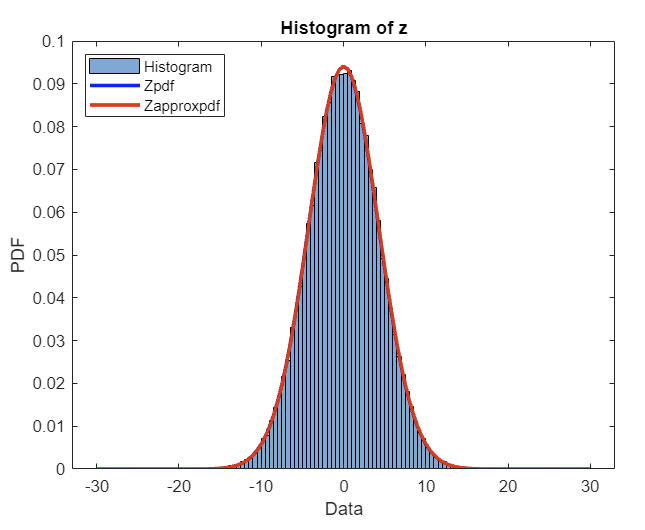
\includegraphics[width=\textwidth]{images/image.png.png}
  \caption{N=10e4}
  \label{2a}
  \end{minipage}
  \hfill
  \begin{minipage}[t]{0.48\textwidth}
  \centering
  \includegraphics[width=\textwidth]{images/n=10e2.png}
  \caption{N=10e2}
  \label{2ab}
  \end{minipage}
  \end{figure}
  

\subsubsection{Does the histogram and two pdfs match well? }

To read the covariance from a PDF curve, find the value of the axis for the peak of the curve and then determine the width of the curve at the half-maximum point, then the width is $ 2 \times \sigma $. 


From figure \ref{2ab}, we can see, when number of points are not enough, we can not achieve the same result as before, the red line which represents the result of \texttt{approxGaussianTransform}  is slightly above blue line which is the theory result, but because we use linear transform now so the result is not too far away.

\subsubsection{From what you see in the figure, what conclusions can you draw regarding the properties of p(z) and the different approximations? }

\begin{itemize}
    \item The analytical and numerical approximations of the transformed Gaussian distribution are very similar in shape, with both pdfs having a peak around zero and a similar spread. This indicates that the numerical approximation using approxGaussianTransform is accurate and provides a good estimate of the true distribution.
    \item Linear transformations preserve the Gaussian nature of the original distribution(Compare with b get this)
\end{itemize}

\subsubsection{How does the number of samples used in the approximation affect the result?}

If the number of samples used in the approximation is small, then the approximation may not be accurate enough to capture the full shape of the probability distribution. As the number of samples used in the approximation increases, the accuracy of the approximation should improve.

\subsection{b}

$$E[z] = E[x^3] = \int x^3 p(x) dx$$

Since x is a normal random variable with mean 0 and variance 2, its probability density function is given by:

$$p(x) = (1 / sqrt(2 * pi * 2)) * exp(-x^2 / 4)
$$

Substituting this into the above equation and evaluating the integral, we get:

$$E[z] = E[x^3] = 0
$$

So, the mean of z is 0.

Next, we can find the covariance of $z$ as follows:

$$Cov[z] = E[(z - E[z])^2] = E[z^2]
$$

To find $E[z^2]$, we can use the following formula:

$$E[z^2] = \int z^2 p(z) dz
$$

where $p(z)$ is the probability density function of $z$.

Substituting $z = x^3$ and using the change of variables formula, we get:

$$E[z^2] = E[x^6] = \int x^6 p(x) dx
$$

To evaluate this integral, we can use the fact that $x^6 = (x^2)^3 $and apply the same technique as before. We get:

$$E[z^2] = E[x^6] = 3 * Var[x]^3 = 3 * 2^3 = 24
$$

Therefore, the covariance of z is:

$$Cov[z] = E[z^2] - E[z]^2 = 24 - 0^2 = 24
$$

So, the mean of z is 0 and the covariance of z is 24.

Draw the picture for PDF and \texttt{approxGaussianTransform}:

\begin{figure}[H]
 \centering
 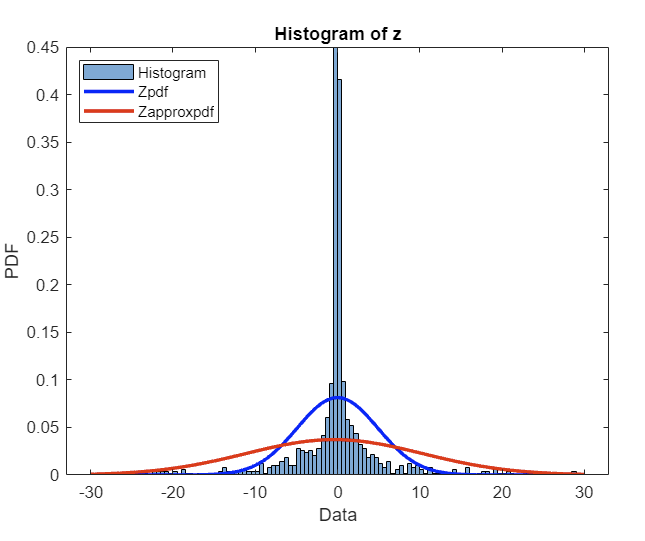
\includegraphics[width=0.7\textwidth]{images/HistogramandPDFcurveforb.png}
 \caption{HistogramandPDFcurveforb}
 \label{2b}
\end{figure}

From the figure \ref{2b}, the blue line discribe the theory normal distribution with the theory mean and covariance that we calculated above.

The red line is the result of \texttt{approxGaussianTransform} , now is totally biased from the theory curve, either the histogram.

So the conclusion for this non-linear part is that the distribution of the Gaussian distribution with non-linear transformation won't be Gaussian distribution.

The \texttt{approxGaussianTransform} method is good for linear situation while it can not be believed in non-linear one.

\subsection{c}

Linear transformations preserve the Gaussian nature of the original distribution while the non-linear transformation may result in a transformed distribution that is not Gaussian, even if the original distribution is Gaussian. This can make it more difficult to estimate the resulting distribution using a Gaussian approximation.

So it is reasonable to use \texttt{approxGaussianTransform} method when facing a linear transformation of Gaussian distribution while shouldn't believe the result of \texttt{approxGaussianTransform} method facing non-linear transformation
